\lecture{Sicurezza negli Stabilimenti Industriali}{26~-~01~-~2026}
%
%
\section{Quadro Normativo}
La sicurezza sul lavoro non è solo una procedura burocratica, ma un obbligo giuridico e morale radicato nella nostra Costituzione e nel Codice Civile. È fondamentale che memorizziate i pilastri legislativi:
\begin{itemize}
    \item \textbf{Costituzione}: L'Art. 32 tutela la salute come diritto fondamentale e l'Art. 41 stabilisce che la libertà d'impresa non può svolgersi in contrasto con l'utilità sociale o recare danno alla sicurezza umana.
    \item \textbf{Codice Civile (Art. 2087)}: Introduce il principio della ``massima sicurezza tecnologicamente fattibile''. L'imprenditore deve adottare tutte le misure che, secondo la particolarità del lavoro, l'esperienza e la tecnica, sono necessarie a tutelare l'integrità fisica e morale dei lavoratori.
    \item \textbf{Codice Penale (Art. 451)}: Punisce l'omissione colposa di cautele contro infortuni e disastri.
    \item \textbf{Evoluzione}: Si è passati da un approccio riparativo (anni '50) a un sistema preventivo e partecipativo con il D.Lgs. 81/2008 (Testo Unico sulla Sicurezza), che armonizza le direttive europee.
\end{itemize}

%
\section{Valutazione dei Rischi}
La gestione della sicurezza segue un processo logico e ciclico che dovete conoscere a menadito (Art. 15 D.Lgs 81/08):
\begin{enumerate}
    \item \textbf{Individuazione e Valutazione}: Si identificano i rischi e si valutano;
    \item \textbf{Misure di Prevenzione}: Si dà priorità alla protezione collettiva rispetto a quella individuale e si cerca di eliminare o ridurre il rischio alla fonte;
    \item \textbf{Attuazione e Partecipazione}: Include formazione, informazione e consultazione dei lavoratori.
\end{enumerate}

Il \emph{Documento di Valutazione dei Rischi (DVR)} è il documento cardine redatto dal Datore di Lavoro (indelebile responsabilità). Deve contenere:
\begin{itemize}
    \item Relazione sulla valutazione di tutti i rischi (inclusi stress lavoro-correlato, differenze di genere, età, provenienza);
    \item Misure di prevenzione e DPI adottati;
    \item Programma di miglioramento nel tempo;
    \item Nominativi delle figure chiave (RSPP, RLS, Medico Competente).
\end{itemize}

%
\section{Ruoli e responsabilità}
In azienda, la sicurezza è un ``gioco di squadra'' con ruoli definiti:
\begin{itemize}
    \item \textbf{Datore di Lavoro (DL)}: Ha l'obbligo di valutare i rischi, designare l'RSPP, fornire DPI, formare i lavoratori e garantire la manutenzione delle attrezzature;
    \item \textbf{Servizio di Prevenzione e Protezione (SPP)}: Insieme di persone/mezzi per individuare rischi e proporre procedure. È ``utilizzato'' dal DL ma ha funzione consultiva tecnica;
    \item \textbf{Rappresentante dei Lavoratori per la Sicurezza (RLS)}: Eletto dai lavoratori, deve essere consultato preventivamente sulla valutazione dei rischi e può fare ricorso alle autorità se ritiene le misure inadeguate;
    \item \textbf{Medico Competente}: Effettua la sorveglianza sanitaria (es. per rischi chimici, VDT, movimentazione carichi);
    \item \textbf{Squadre di Emergenza}: Lavoratori formati per antincendio, evacuazione e primo soccorso.
\end{itemize}
Inoltre, nell'ambito istituzionale, sono presenti organi di vigilanza, che controllano e mitigano il pericolo, e se necessario soccorrono:
\begin{itemize}
    \item \textbf{ASL}: Accerta violazioni, cause di infortuni e verifica la rispondenza alle norme;
    \item \textbf{INAIL}: Ente tecnico-scientifico, fornisce consulenza e omologa prodotti industriali;
    \item \textbf{Vigili del Fuoco (VVF)}: Rilasciano il Certificato di Prevenzione Incendi (CPI) e controllano attività a rischio esplosione/incendio.
\end{itemize}

%
\section{Movimentazione Manuale dei Carichi}
Questo è un argomento tecnico di alta importanza. Si applica il metodo NIOSH.
%
\paragraph{Costante di Peso} Il peso ideale sollevabile in condizioni ottimali varia in base alla popolazione. Secondo la proposta EPM basata su UNI EN 1005-2:
\begin{itemize}
    \item Maschi (18-45 anni): $ 25 \si{\kg} $;
    \item Femmine (18-45 anni): $ 20 \si{\kg} $ (alcune tabelle indicano $ 15 \si{\kg} $ per protezione maggiore o età diverse).
\end{itemize}

%
\paragraph{Calcolo del Peso Limite Raccomandato} Per calcolare il PLR utilizziamo la costante di peso $ CP $:
\[
    PLR = CP \cdot A \cdot B \cdot C \cdot D \cdot E \cdot F
\]
Dove i fattori (tutti $ \leq 1$) penalizzano (demoltiplicazione) il sollevamento se:
\begin{itemize}
    \item A (Altezza): Le mani non sono ad altezza ideale (75 cm);
    \item B (Dislocazione): Lo spostamento verticale è ampio;
    \item C (Orizzontale): Il peso è lontano dal corpo;
    \item D (Asimmetria): C'è torsione del busto;
    \item E (Presa): La presa è scarsa;
    \item F (Frequenza): I sollevamenti sono frequenti.
\end{itemize}
Vedi figura \ref{fig:niosh1}.

%
\paragraph{Indice di Sollevamento/Rischio}
\[
    IS = \frac{\text{Peso Sollevato Reale}}{PLR}
\]
Se:
\begin{itemize}
    \item $ IS < 0.85 $: Il rischio è trascurabile;
    \item $ 0.86 < IS < 0.99 $: Richiede attenzione;
    \item $ IS \geq 1 $: Rischio presente/alto, trattare immediatamente.
\end{itemize}
Vedi figura \ref{fig:niosh2}.

\begin{figure}
    \centering
    \begin{subfigure}{0.45\linewidth}
        \centering
        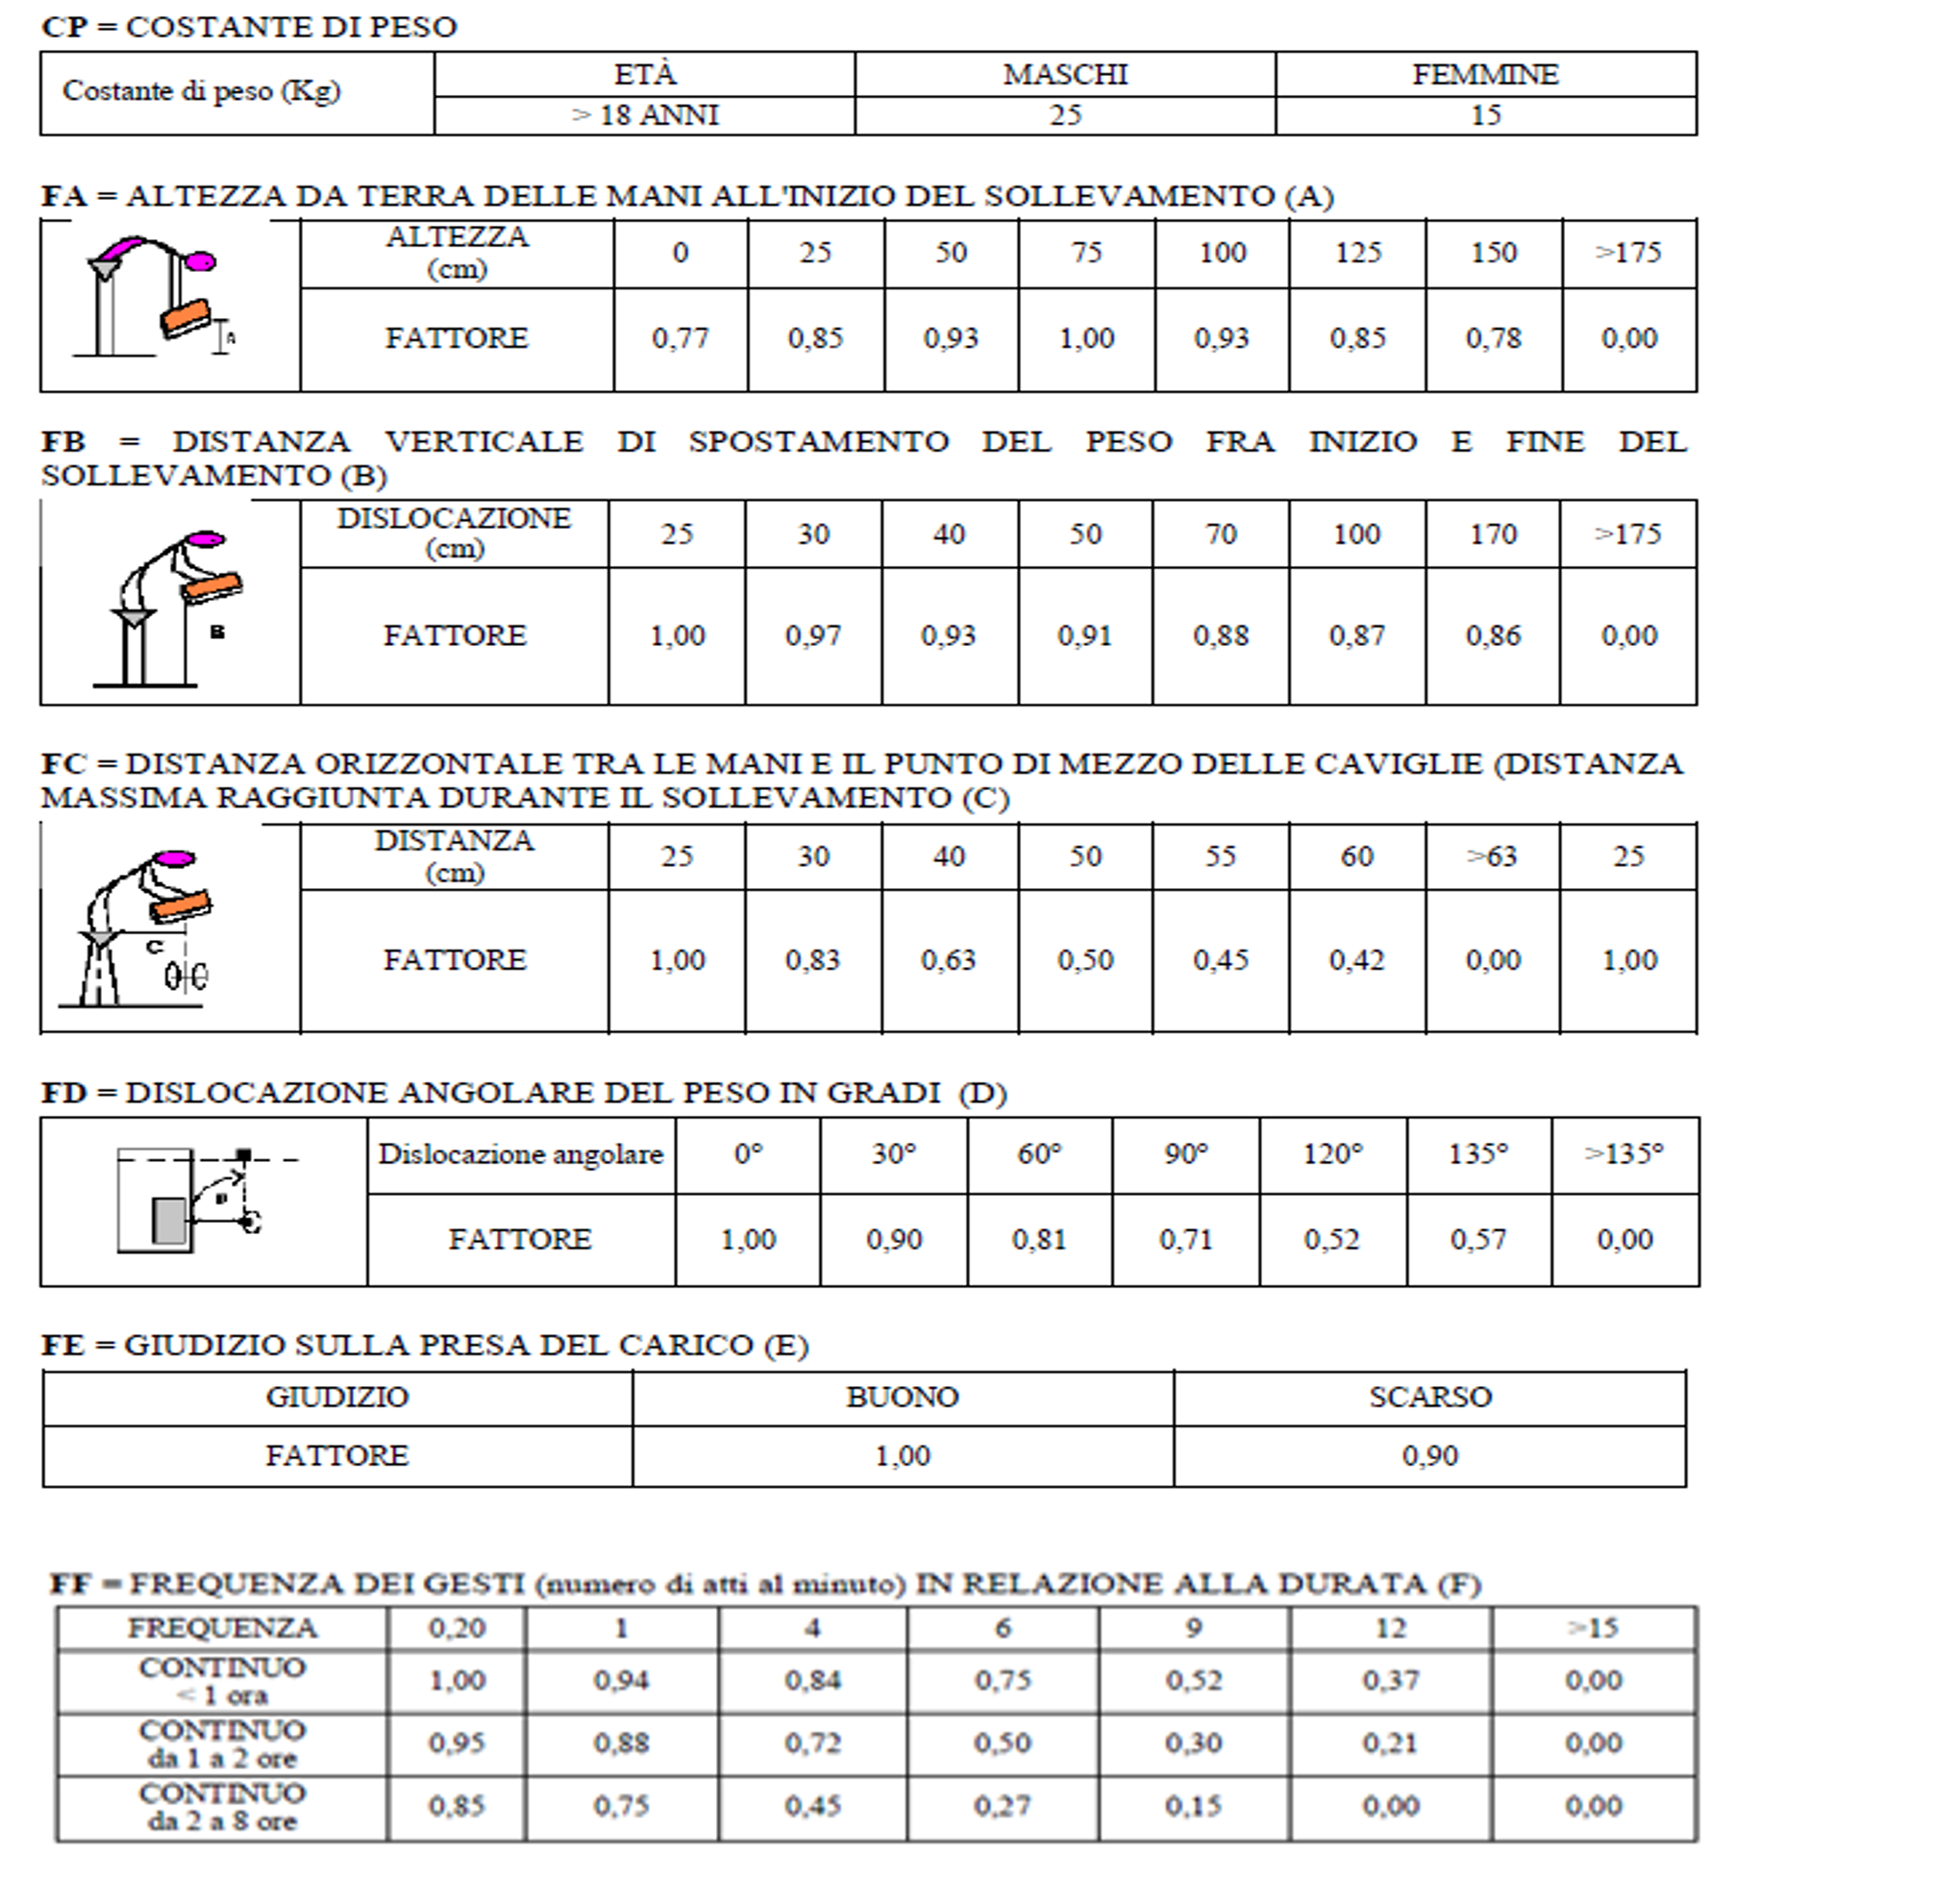
\includegraphics[width=\linewidth]{assets/29.png}
        \caption{Metodo NIOSH-1}\label{fig:niosh1}
    \end{subfigure}
    \begin{subfigure}{0.45\linewidth}
        \centering
        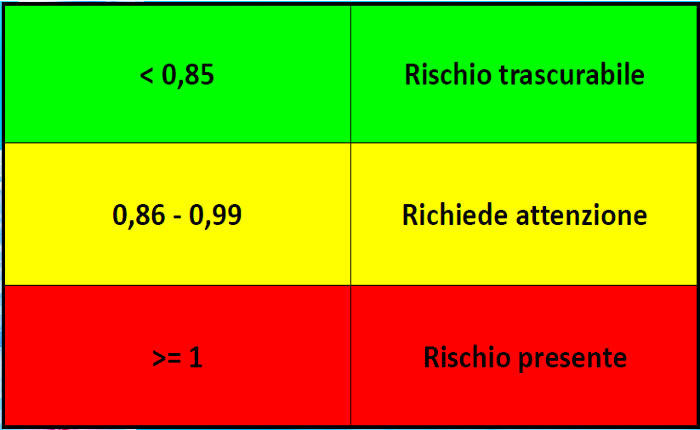
\includegraphics[width=\linewidth]{assets/30.png}
        \caption{Metodo NIOSH-2}\label{fig:niosh2}
    \end{subfigure}
\end{figure}

%
\paragraph{Principi Ergonomici}
\begin{itemize}
    \item Evitare torsioni del busto e sollevamenti da terra a schiena flessa;
    \item Mantenere il carico vicino al corpo;
    \item Progettare postazioni con angoli di prelievo/deposito max 90° (mai 180°);
    \item Utilizzare ausili (piattaforme a pantografo, ventose) per mantenere il carico ad altezza fianchi (60-80 cm).
\end{itemize}

%
\section{Requisti dei luoghi di lavoro e segnaletica}
La sicurezza strutturale è la prima forma di prevenzione.
%
\paragraph{Requisiti Dimensionali}
\begin{itemize}
    \item Altezza netta $\geq 3 \si{\m}$;
    \item Cubatura $\geq 10 \si{\m^3}$ per addetto;
    \item Superficie $\geq 2 \si{\m^2}$ per addetto;
\end{itemize}

%
\paragraph{Vie di Circolazione}
\begin{itemize}
    \item Separare il traffico pedonale da quello veicolare (muletti);
    \item Se coesistono, garantire una distanza di sicurezza per i pedoni ($\approx 70 \si{\cm} $);
    \item Usare sbarramenti o strisce gialle/bianche per delimitare le zone.
\end{itemize}

%
\paragraph{Vie di Emergenza}
\begin{itemize}
    \item Devono aprirsi nel verso dell'esodo (maniglione antipanico) e avere altezza minima $ 2 \si{\m} $;
    \item Lunghezza massima percorsi:
          \begin{itemize}
              \item Rischio elevato: 15-30 m;
              \item Rischio medio: 30-45 m;
              \item Rischio basso: 45-60 m.
          \end{itemize}
\end{itemize}

%
\paragraph{Segnaletica di Sicurezza (Colori e Forme)}
\begin{enumerate}
    \item \textbf{Rosso} (Quadrato/Rotondo): Materiale antincendio o Divieto;
    \item \textbf{Giallo/Arancio} (Triangolare): Avvertimento/Pericolo;
    \item \textbf{Azzurro} (Rotondo): Prescrizione (es. obbligo caschetto/cuffie);
    \item \textbf{Verde} (Quadrato/Rettangolare): Salvataggio, Uscite di sicurezza, Primo soccorso.
    \item \textbf{Giallo/Nero} (Strisce): Segnalazione ostacoli fissi.
\end{enumerate}

%
\section{Rischi Specifici: Epidemie e Stress}
%
\paragraph{Prevenzione Contagi} Utilizzare tecnologie come l'RTLS (Real Time Locating System) con tag UWB per monitorare il distanziamento sociale in tempo reale, garantendo la privacy (tag anonimi). Implementare checklist pre-turno e dispenser di DPI.
%
\paragraph{Stress Lavoro-Correlato} Attenzione ai fattori psicosociali: rapporto conflittuale uomo-macchina, carico di lavoro eccessivo o scarso, monotonia, responsabilità non calibrate e fattori ambientali (rumore).